%!TEX TS-program = xelatex
%!TEX encoding = UTF-8 Unicode

\documentclass[12pt]{extarticle}
% extarticle is like article but can handle 8pt, 9pt, 10pt, 11pt, 12pt, 14pt, 17pt, and 20pt text

\def \ititle {Philosophical Psychology}

\def \isubtitle {Lecture 05}

\def \iauthor {Stephen A. Butterfill}
\def \iemail{s.butterfill@warwick.ac.uk}
\date{}

%for strikethrough
\usepackage[normalem]{ulem}

\input{$HOME/latex_imports/preamble_steve_handout}

%\bibpunct{}{}{,}{s}{}{,}  %use superscript TICS style bib
%remove hanging indent for TICS style bib
%TODO doesnt work
\setlength{\bibhang}{0em}
%\setlength{\bibsep}{0.5em}


%itemize bullet should be dash
\renewcommand{\labelitemi}{$-$}

\begin{document}

\begin{multicols*}{3}

\setlength\footnotesep{1em}


\bibliographystyle{newapa} %apalike

%\maketitle
%\tableofcontents




%---------------
%--- start paste




\def \ititle {Lecture 05: The Developmental Origins of Knowledge of Physical Objects}

\begin{center}

{\Large

\textbf{\ititle}

}



\iemail %

\end{center}


‘... ’tis past doubt, that Men have in their Minds several Ideas ...: It is in the first place to be enquired, How he comes by them?’ \citep[p.~104]{Locke:1975qo}.

What is the nature of infants’ earliest cognition of physical objects?
And how do you get from these early forms of cognition to
knowledge of simple facts about particular physical objects?

\section{4- and 5-month-olds can track briefly occluded objects}

\begin{center}
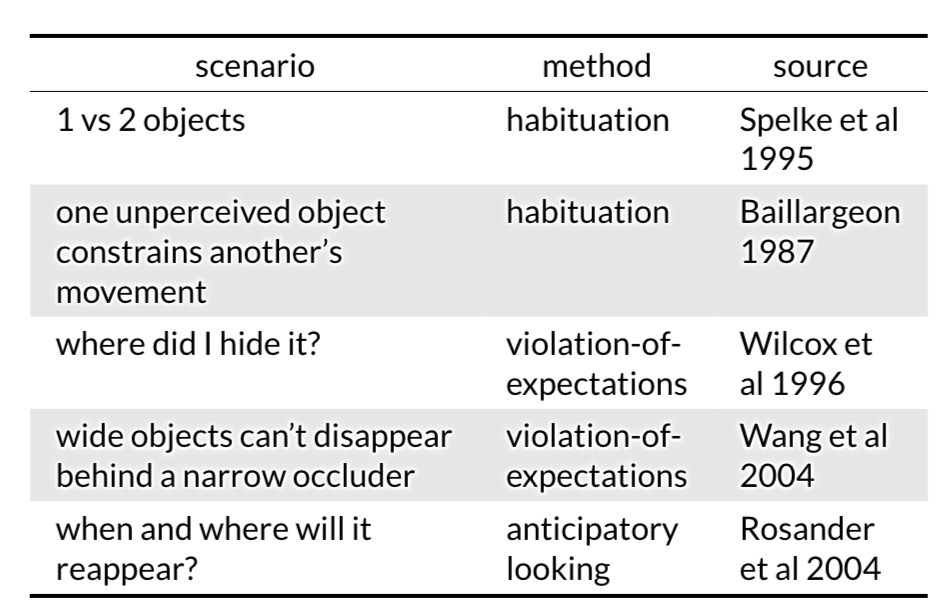
\includegraphics[width=0.3\textwidth]{fig/table1.png}
\end{center}

For a process to \emph{track} an occluded object
is for it to nonaccidentally  depend in some way on
the occluded object’s path.


\section{Core Knowledge}
‘there is a third type of conceptual structure, dubbed “core knowledge” ... that differs systematically from both sensory/perceptual representation[s] ... and ... knowledge.’
\citep[p.~10]{carey:2009_origin}

‘core systems are
largely innate,
encapsulated,
unchanging,
arising from phylogenetically old systems, [and]
built upon the output of innate perceptual analyzers’
\citep[p.~520]{Carey:1996hl}.



\section{The CLSTX Conjecture}

Four- and five-month-olds' abilities to track briefly unperceived objects
are not grounded on belief or knowledge:
instead
they are consequences of the operations of
a system of object indexes.
\citep{Leslie:1998zk,Scholl:1999mi,Carey:2001ue,scholl:2007_objecta,carey:2009_origin}.

An \emph{object index} is ‘a mental token that functions as a
pointer to an object’ \citep[p.\ 11]{Leslie:1998zk}.

The \emph{object-specific preview benefit} is the reduction in time needed to identify that a letter (or other feature) matches a target presented earlier when the letter and target both appear on the same object rather than on different objects.

Object indexes ...
\begin{itemize}
\item guide ongoing action (e.g.~visual tracking, reaching)
\item influence how attention is allocated
\citep{flombaum:2008_attentional}
\item can be assigned in ways incompatible with beliefs and knowledge \citep[e.g.][]{Mitroff:2004pc, mitroff:2007_space}
\item have behavioural  and neural markers, in adults and infants   \citep{richardson:2004_multimodal,kaufman:2005_oscillatory}.
\item are subject to signature limits \citep[pp.~83--87]{carey:2009_origin}
\item sometimes survive occlusion \citep{flombaum:2006_temporal}
\end{itemize}

A \emph{signature limit of a system} is a pattern of behaviour the system exhibits which is both defective given what the system is for and peculiar to that system.


\section{Objects Represented Motorically}
In adults, merely observing a handled object that appears within reach produces brain activity linked to the hand with which it could most readily be grasped \citep{cardellicchio:2011_space}.

Putting a barrier (even a translucent one) between you and a graspable object eliminates or greatly reduces the tendency to represent the object motorically \citep[e.g.][]{costantini:2010_where}.

\emph{Revised CLSTX Conjecture}:
Four- and five-month-olds' abilities to track briefly unperceived objects are also consequences of a further, independent capacity to track physical objects which involves motor representations and processes.

Prediction: When occluders and barriers are deconfounded, infants’ performance is consistent with the Revised CLSTX Conjecture (see \citealp{mccurry:2009_beyond}).

\vfill


\footnotesize
\bibliography{$HOME/endnote/phd_biblio}

\end{multicols*}

\end{document}
